%!TEX encoding = UTF-8 Unicode
% !TeX spellcheck = en_GB
\chapter{Higgs Physics }\label{chap:HiggsPhys}
%%
\section{Spontaneous symmetry breaking}
\par Before talking about symmetry breaking, we need to discuss the concept of symmetry in physics. Symmetry has an essential role in studying physical systems. It manifests not only as a geometric feature of physical objects but also in the dynamics of physical systems. For example, one can find symmetries in the equation of motion, Lagrangians/Hamiltonians and actions. The magnetisation of materials is a good example of the role that symmetry plays in describing physical behaviour. For instance, \textbf{paramagnetic} materials have a positive magnetic susceptibility~$\chi_B$ due to the random arrangement of their electrons' spins.  The paramagnetic material spins arrangement will therefore possess rotational symmetry. The material has no \textit{ preferred direction} in space~\cite{minlos2000introduction}. On the contrary, \textbf{ferromagnetic} materials with the electrons' spins aligned in a certain direction, will not have such symmetry as there will be a preferred direction, see~\autoref{fig:paravsferro}. 
%%%%
\begin{figure}[htpb!]
    \centering  
   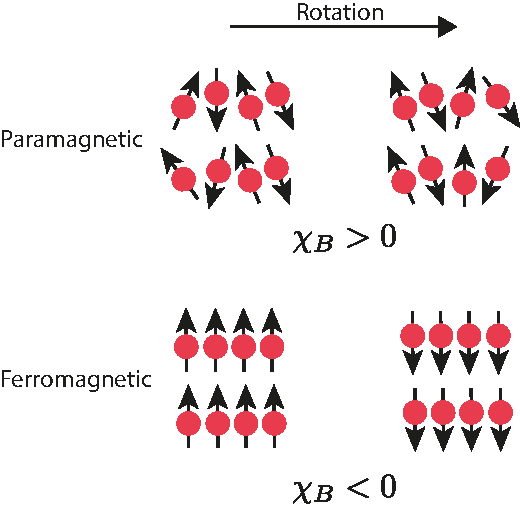
\includegraphics[width=0.36\linewidth]{./figures/ferrvspara}
    \caption{In paramagnetic materials, the spins are randomly distributed such that a rotation performed on the system will keep the spin distribution invariant. However, for ferromagnetic materials, where the spins are aligned in a single direction, the symmetry is broken, and the system has a preferred direction.}  \label{fig:paravsferro}
\end{figure}
%%%%
%%%%
\par In particle physics and quantum field theory, symmetry plays an essential role in the taxonomy and dynamics of elementary particles and their bound states, i.e. hadrons, cf.~\cite{osti_4008239,PhysRev.96.191}. There are two types of symmetries considered when studying elementary particles and their quantum fields: external and internal symmetries. The first is the symmetry of the spacetime background. Typically, this is a four-dimensional Poincar\'e symmetry. However, in some models, higher spacetime dimensions or non-flat geometries are considered. Though there is no current evidence of higher dimensions or indications of non-flat spacetime from colliders and cosmological observations~\cite{Zyla:2020zbs}. The second class of symmetries is internal symmetries stemming from the quantum nature of these particles/fields. Because their state is described by a \textbf{ray} in complex Hilbert/Fock spaces, internal symmetries are simply symmetries of rotations in these spaces that keep the action variation unchanged. Internal symmetries are usually described in terms of simple or product of simple \textbf{Lie groups}, e.g. $SU(N)$~\footnote{Gauge theories based on finite groups have been investigated in the literature, but their phenomenological significance is yet to be further investigated~\cite{Freed1993LecturesOT,dijkgraaf1990topological}}, and particles/fields will be arranged as multiplets in some representation of the groups. The rotations of the states could be parametrised by constants. In this case, the symmetry is called \textbf{global}, or fields of spacetime, where the symmetry is then called \textbf{local} or \textbf{gauged}.
%%%%
\par Gauge symmetries describe rotations in the state space that depend on spacetime, the generator of the gauge transformations could propagate between two spacetime points. This is the way particle/field interactions are described in quantum field theory. The generators of these gauge transformations are called gauge bosons, and they mediate the interactions between the particles/fields and transform under the adjoint representation of the gauge group. Hence, we observe that gauge symmetries are the basis of describing the fundamental interactions of nature, which we call \textbf{gauge theories}.
%%%%
\par An example of a gauge theory that is realised in nature is the \textbf{Standard Model}~(SM). Which is a gauge theory based on the group~$G_{\SM}:=SU(3)_C \otimes SU(2)_L \otimes U(1)_Y$. The first simple group is for the \textit{strong} interaction described by quantum chromodynamics~(QCD). The product of the two remaining groups~$SU(2)_L \otimes U(1)_Y$ forms the Weinberg-Salam \textit{electroweak}~(EW) model~\cite{salam1,salam2,PhysRevLett.19.1264}, where~$SU(2)_L$ describes the weak interaction which only couples to \emph{left handed} fermions and $U(1)_Y$ is the weak hypercharge~$Y$ gauge group, defined by the formula
\begin{equation}
    Y= 2(Q-T_3).
\end{equation}
Where $Q$ is the electric charge and $T_3$ is the third component of the weak isospin. A description of the matter content of the SM and their multiplicities with respect to~$G_{\SM}$ is shown in~\autoref{tab:thesm}
%%%%
\begin{table}[htpb!]
    \centering
    \begin{tabular}{ccc}
        \toprule
         Particle/Field& $G_\SM$ multiplicity& mass [\si{\GeV}] \\
         \midrule
         $Q = {u_L \choose d_L},{c_L \choose s_L},{t_L \choose b_L}$ & $(\irrep{3},\irrep{2},1/6)$ & $m_u=2.16\cdot10^{-3}$, $m_d=2.67\cdot10^{-3}$\\
         $U= u_R, s_R, t_R$ & $(\irrep{3},\irrep{1},2/3)$&$m_c=0.93\cdot10^{-2}$, $m_s=1.27$\\
         $D= d_R, s_R, b_R$ & $(\irrep{3},\irrep{1},-1/3)$&$m_t=172.4$, $m_b=4.18$\\
         \midrule
         $L = {\nu_{e,L} \choose e_L},{\nu_{\mu,L} \choose \mu_L},{\nu_{\tau,L} \choose \tau_L}$ & $(\irrep{1},\irrep{2},-1/2)$ & $m_e=0.511\cdot10^{-3}$, $m_\mu=1.05\cdot10^{-2}$\\
         $E= e_R, \mu_R, \tau_R$ & $(\irrep{1},\irrep{1},-1)$&$m_\tau=1.77$,$m_\nu=$??\\
         \midrule
         $g/G^A_\mu,\,\,\, A=1\dots 8$ &$(\irrep{8},\irrep{1},0)$&$ 0.0$\\
         $\gamma/A_\mu$ &$(\irrep{1},\irrep{1},0)$&$ 0.0$\\
         $W^\pm_\mu$ &$(\irrep{1},\irrep{3},0)$&$ 80.379$\\
         $Z_\mu$ &$(\irrep{1},\irrep{3},0)$&$ 91.1876$\\
         \midrule
         $h$ &$(\irrep{1},\irrep{2},1/2)$&$ 125.10$\\
        \bottomrule
    \end{tabular}   
        \caption{The SM constituents, their multiplicities with respect to the SM gauge group ~$G_{\SM}:=SU(3)_C \otimes SU(2)_L \otimes U(1)_Y$ and masses. The mass of the neutrinos $\nu$ is zero according to the SM prediction, but observations suggest that they are massive, and only the difference between the three masses is known~\cite{Capozzi:2016rtj}. The values of the masses are taken from the Particle Data Group~(PDG)~\cite{Zyla:2020zbs}, and used throughout this thesis.}\label{tab:thesm}
\end{table}

%%%%
%%%%
\par The SM has been very successful at describing particle interactions even when challenged by numerous precision tests at LEP and SLD~\cite{ALEPH:2005ab,SLD:2000jop,Group:2012gb,ALEPH:2013dgf} and later at D\O~\cite{2011baz} and the LHC~\cite{CMS:2014mgj,ATLAS:2017rzl} Nevertheless, it fails to describe the ground state if only the fermion and gauge sectors are considered. The reason for this shortcoming is that the $W^\pm$ and $Z$ bosons have a mass, this violates the EW gauge symmetry. This can be easily seen by looking at the mass term of a spin 1 field $B^A_\mu$
\begin{equation}
    \mathcal{L} = m_B B^{A,\mu}B^A_\mu,
\end{equation}
and performing an $SU(N)$ gauge transformation 
\begin{equation}
    B^A_\mu \to B^A_\mu+\partial_\mu \Lambda ^A+g \,\varepsilon^A_{BC} B^B_\mu \Lambda^C.
\end{equation}
We see that the mass term is invariant under these transformations.
Secondly, because the SM is a chiral theory, as only left-handed fermions would be doublets under~$SU(2)_L$, the Dirac mass term
\begin{equation}
    \mathcal{L}_{\mathrm{D}} = m_D \bar \psi_L \psi_R+ \hc,
\end{equation}          
cannot be a singlet under~$SU(2)_L$, hence also violating the EW symmetry. Despite quark and lepton masses being forbidden by the EW symmetry, we indeed observe that they do have a mass, and since they also carry charges this mass has to be a Dirac mass. 
\par In order for the EW model to be consistent at the ground state like it is in the interaction states. A mechanism for spontaneous symmetry breaking going from an interaction state to the vacuum ought to be introduced. 
%%%%%%
\subsection{Nambu-Goldstone theorem}
%%%%%%%
Coming back to the example of the paramagnetic-ferromagnetic materials, when heated above a certain temperature, known as the~\textbf{Curie Temperature}~$T_C$ will undergo a phase transition and become paramagnetic~(losing their permanent magnet property), in the mean-field theory approximation the magnetic susceptibility is related to the temperature of the metal via the relation
\begin{equation}
    \chi_B \sim (T-T_C)^{-\gamma},
\end{equation}  
where $\gamma$ is a critical exponent. We see that if the metal temperature $T>T_C$ the metal is in an~\textit{disordered phase} and when $T<T_C$ it is in the~\textit{ordered phase},i.e. $\chi_B$ is the \textbf{order parameter} of this system. At the Curie temperature, the system will be at the~\textit{critical point} where the susceptibility is divergent. The exponent $\gamma$ is not used to describe the system at the critical point. There is a ``pictorial'' description of the metal at the critical point which is helpful in picturing the Goldstone theorem. Starting at $T>T_C$, the metal would be in a paramagnetic phase, where the spins are randomly arranged. As the temperature becomes lower and lower, thermal fluctuations start to lessen.  One or more regions of the metal, some of the spins will start to get aligned With continued cooling, nearing $T_C$, these turned spins will affect their neighbours turning them into their directions. At the critical point $T=T_C$, the system behaves in a peculiar manner, when one would see regions of spins in ``up'' and others in ``down'' directions. The system will resemble a fractal of these regions, becoming scale-invariant. Additionally, waves of oscillating local magnetisation will propagate. These waves, or spinless quasiparticles (called \textbf{Magnons}) are Goldstone bosons emerging from spontaneous symmetry breaking. Which will manifest at $T<T_C$ as the spins will be  arranged in a certain single direction and the metal becomes ferromagnetic.
\begin{theorem}[Nambu-Goldstone]
    When a continuous symmetry has a conserved currents but broken in the ground state~(vacuum) is called to be spontaneously broken. There is a scalar boson associated with each broken generator of this spontaneously broken symmetry. The modes of these bosons are fluctuations of the order parameter.
\end{theorem}
This theorem first emerged from condensed matter physics, particularly superconductors~\cite{PhysRev.117.648,goldstone}. However, it soon got applied to relativistic quantum field theories~\cite{PhysRev.127.965}.
%%%%%%
\subsection{The Higgs mechanism}
%%%%%%
In order to solve the aforementioned shortcomings of the Weinberg-Salam model, Nambu-Goldstone theorem has been first proposed by P.~W.~Anderson~\cite{PhysRev.130.439}. However, the way that Anderson formulated his theory was unfamiliar to particle physicists and used a non-relativistic picture to illustrate how photons could gain mass in an electron plasma with a plasma frequency $\omega_{p}$ 
\begin{equation}
    m_\gamma^{\mathrm{plasma}} =\frac{\hbar \omega_p}{c^2}
\end{equation}
Later on, a theory that explains the mass generation of the EW gauge bosons has been published in an almost simultaneous manner by R.~Braut~ and F.~Englert~\cite{PhysRevLett.13.321}, P.~Higgs~\cite{PhysRevLett.13.508} and G.~Guralnik, C.~R.~Hagen, and T.~Kibble~\cite{PhysRevLett.13.585,Guralnik:2009jd}\footnote{All of these authors have contributed to the theory of SM spontaneous symmetry breaking~(SSB). By calling it the ``Higgs'' mechanism or boson. I, by no means, have intended to ignore the role played by the rest, rather, I wanted to stick the most widely-used terminology in the field.}.
The Higgs mechanism starts by considering the spontaneous symmetry breaking~(SSB) of the EW sector of the SM via the pattern
\begin{equation}
    SU(2)_L \otimes U(1)_Y \longrightarrow U(1)_{Q} 
\end{equation}
This is  achieved by the vacuum expectation value~(vev) of a complex scalar field $\phi\sim (\irrep{1},\irrep{2},+1/2)$, with the Lagrangian 
\begin{equation}
    \mathcal{L} = D_\mu \phi^* D^\mu \phi -V,\;\;\;\;\;\; V:= \mu^2  \phi^* \phi +\lambda (\phi^* \phi)^2,
    \label{higgspot}
\end{equation}
 were $\phi$ is given explicitly by 
 \begin{equation}
  \phi = \begin{pmatrix}
      \phi^1 + i \phi^2\\  \frac{1}{\sqrt{2}}(h+v)-i \phi^3
  \end{pmatrix}
\end{equation}
The covariant derivative 
\begin{equation}
    D_\mu= \partial_\mu -ig_2\frac{\sigma_a}{2}W^a_\mu-ig_1\frac{1}{2} B_\mu,   
\end{equation}
dictates the coupling between the Higgs field and the EW gauge bosons and~$g_3$, $g_2$ and $g_1$ are, respectively, the coupling constants of 
${ SU(3)_C}$,  ${ SU(2)_L}$ and  ${ U(1)_Y}$.  
 The minimum of the scalar potential is then obtained by
 \begin{equation}
\frac{\partial V}{\partial \phi} \mid_{\phi\to v} = 0,
\end{equation}
which for a tachyonic mass~$\mu^2 < 0$ will have a real non-vanishing values~$v$ corresponding to the vev of this field~$\langle \phi \rangle ={0\choose \frac{v}{\sqrt{2}}}$.\\
According to Nambu-Goldstone theorem, the three broken generators of~$SU(2)_L \otimes U(1)_Y$ will become massive, and they are the $W^\pm$ and $Z$ bosons, while the photon will remain massless. We will have three massless Goldstone bosons $ G^\pm=\frac{1}{2} (\phi^1\pm i\phi^2) $ and $G^0=\phi^3$ that are ``eaten'' by the aforementioned massive photons. Where they become the longitudinal polarisations of $W^\pm$ and $Z$ boson. In order to see this more concretely, we start by looking at the terms of the EW Lagrangian where the field $\phi$ couples to the gauge bosons, in the unbroken phase
\begin{equation}
   D_\mu \phi^* D^\mu \phi = \frac{1}{2} |\partial_\mu \phi|^2 + \frac{1}{8}g_2^2|\phi|^2|W_\mu^1+iW_\mu^2|^2
   + \frac{1}{8}|\phi|^2 |g_2 W_\mu^3- g_1 B_\mu|^2
   \label{ewhiggs_ub}
\end{equation}
After SSB, we write the gauge bosons in the mass basis~
\begin{align}
W_\mu^\pm &= \frac{1}{\sqrt{2}} (W^1_\mu\pm iW^2_\mu), \nonumber \\
Z_\mu &= \frac{1}{\sqrt{g_1^2+g_2^2}} \left(g_2 W^3_\mu-g_1B_\mu\right), \\
A_\mu &= \frac{1}{\sqrt{g_1^2+g_2^2}} \left(g_2 W^3_\mu+g_1B_\mu\right). \nonumber
 \end{align}
 From this, the electric change is identified as the coupling constant to the photon~$A_\mu$ 
 \begin{equation}
     e=\frac{g_1}{\sqrt{g_1^2+g_2^2}}
 \end{equation}
and we use the unitary gauge 
\begin{equation}
    \phi \to \begin{pmatrix}
       0\\  \frac{1}{\sqrt{2}}(h+v).
    \end{pmatrix}, \,\,\,\,\,\,\,\, v= 246\, \mathrm{GeV}.
    \label{unitaryhiggs}
  \end{equation}
With these substitutions, one can read off the masses of the gauge bosons their bilinear terms in~\eqref{ewhiggs_ub}
\begin{align}
    m_W =& \frac{vg_2}{2} & m_Z&=\frac{v}{2}\sqrt{g_1^2+g_2^2} & m_A &= 0.
\end{align}
Since $\phi$ is a complex doublet. We have seen that it has four components,  and three of them correspond to the Goldstone bosons, thus one remains physical~$h$ which is what we now identify with the ``Higgs boson'' discovered in the Summer of 2012. The couplings between  the Higgs and the electroweak bosons is related to their mass via the vev 
\begin{align}
    g_{hVV} =& \frac{2 m_V^2}{v}, & g_{hhVV}=& \frac{2 m_V^2}{v^2}.
\end{align}
By substituting~\eqref{unitaryhiggs}, into the Higgs potential~\eqref{higgspot} one can write the mass of the physcial Higgs boson in terms of the vev
\begin{align}
  m_h =\sqrt{2 \lambda} v.
\end{align}
One could also identify the self-couplings of~$h$, the trilinear and quartic couplings 
\begin{align}
    g_{hhh}&=3\lambda v =3\frac{m_h^2}{v}, & g_{hhhh}&= 3 \lambda = 3\frac{m_h^2}{v^2}.
\end{align}
%%%
\subsection{Yukawa interaction}
It is possible to also use the Higgs vev to give fermions their masses by introducing a Yukawa-interaction terms, first introduced by S. Weinberg~\cite{PhysRevLett.19.1264}
\begin{equation}
    \mathcal{L}_{\mathrm{Yuk}}= -y_{e} \, \bar{L} \, \phi \, E 
- y_{d} \, \bar{Q} \, \phi \, D
- y_u \, \bar{Q} \, \tilde{\phi} \, U   \ + \hc,
\end{equation}
with $ \tilde{\phi}= i\sigma_2 \phi$ and $ y_e, y_d, y_u$ are $3\times 3$ matrices. These matrices are free parameters in the SM. As the Higgs boson acquires a the vev, the fermions will acquire a mass $m_f= vy^\prime_f$ and the Higgs boson coupling to the fermions is given by
\begin{equation}
	g_{h\bar{f}f} = \frac{m_f}{v},
\end{equation}
 and the Yukawa matrices will be fixed in the mass basis ~$y^\prime_f$ by measurements of the fermion masses.\\  Leptonic Yukawa matrix is diagonal, with a degeneracy between the flavour and masses basis, this manifests as lepton family number conservation~(the lepton family operator commutes with the Hamiltonian.). However, for the quarks, the situation is more complicated. One can rotate these matrices to the mass basis via a bi-unitary transformation via the unitary matrices~$ \mathcal{V}_Q, \mathcal{U}_Q$ for $ q= u,d$
\begin{equation}
    y_{q} \longrightarrow y^\prime_f= \mathcal{V}^\dagger_{q} \,y_q\, \mathcal{U}_{q} = \text{diag}\left(m_{q_1}, m_{q_2},m_{q_3}\right).
\end{equation}
However, the is no degeneracy here, the Hamiltonian does not commute with the quark flavour operator. This is because the transformation matrices for the up and down-type quarks are not the same.  The charged EW quark currents contains flavour mixing described by the Kabibbo-Kobayashi-Maskawa~(CKM) matrix~\cite{PhysRevLett.10.531,10.1143/PTP.49.652}. More details on the flavour sector of the SM is discussed in~\la{Update the section}\\
\autoref{fig:SMcouplings} shows all the SM couplings' strengths, with the thickness of the chord is proportional to the strength of the coupling, on can see the Higgs couplings in orange. 
%%%%
\begin{figure}[htpb!]
    \centering
    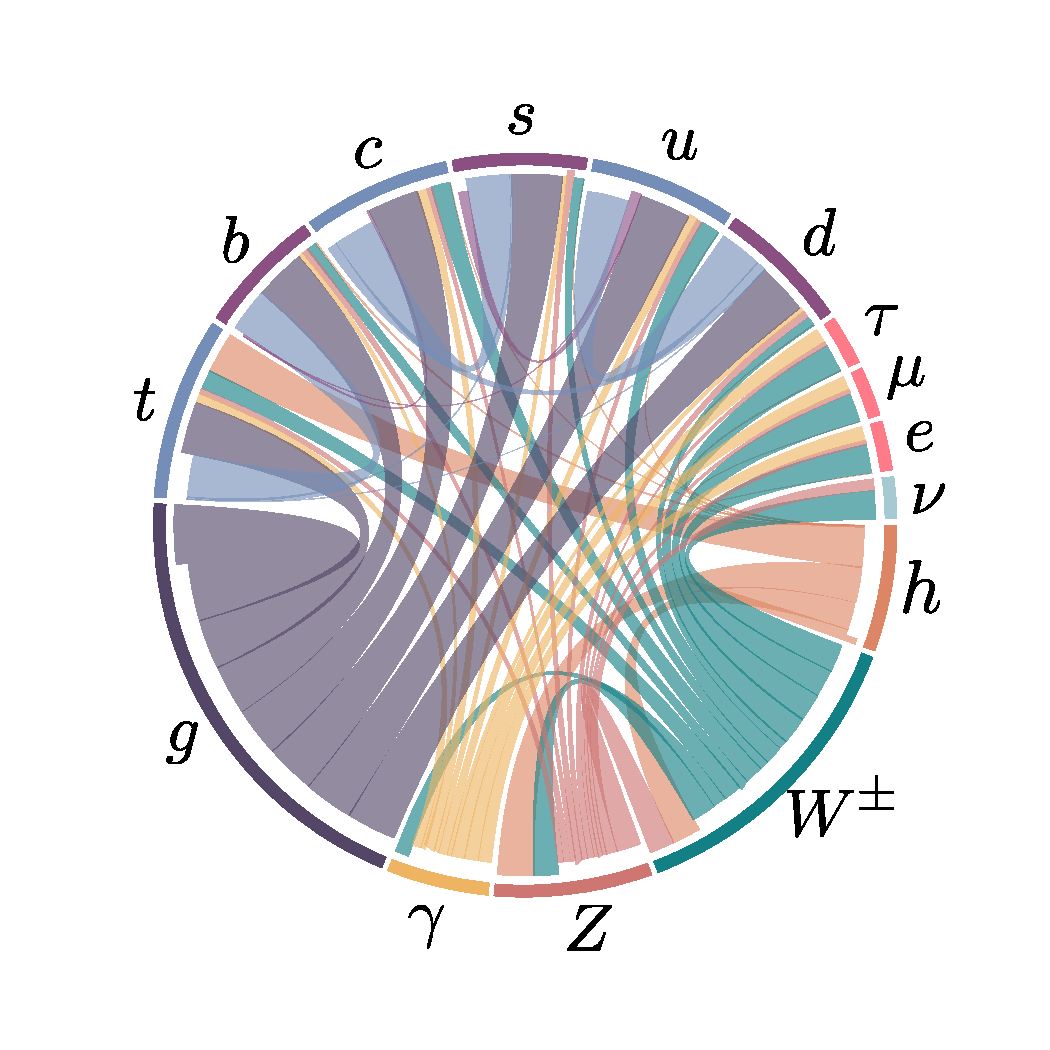
\includegraphics[width=\linewidth]{./figures/SM}
    \caption{A chord diagram showing the SM couplings, with the coupling strength illustrated by the chord thickness. Higgs couplings are coloured in orange.}  \label{fig:SMcouplings}
\end{figure}
%%%%
%%%%
\section{Theoretical constraints on the Higgs}
